\documentclass[tikz,border=4pt]{standalone}
\usepackage{tikz}
\usepackage{polymer-paper-preamble}

\usetikzlibrary{arrows.meta,calc,decorations.pathmorphing,patterns}

\begin{document}
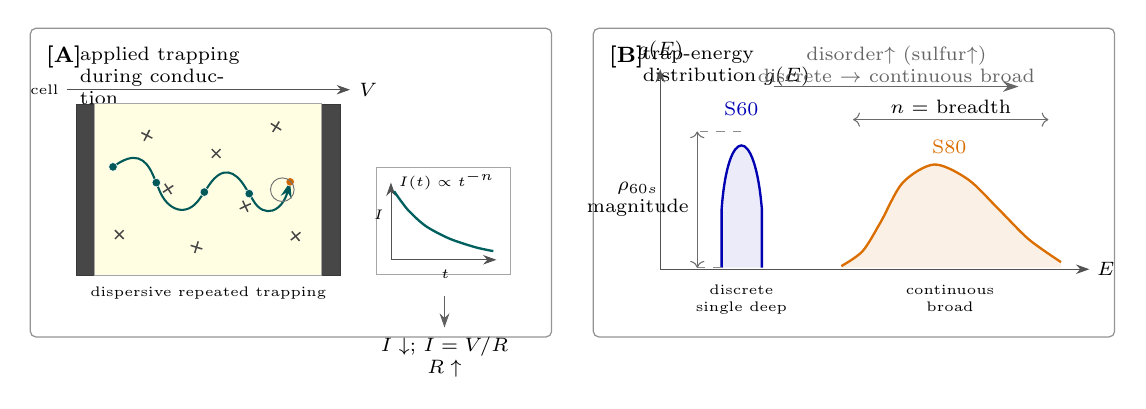
\begin{tikzpicture}[
  x=1cm,y=1cm,
  font=\sffamily,
  panel/.style={draw=black!42, line width=0.45pt, rounded corners=2pt},
  label/.style={font=\bfseries\footnotesize, inner sep=1pt},
  small/.style={font=\scriptsize, inner sep=1.2pt},
  tinytxt/.style={font=\tiny, inner sep=1pt},
  electrode/.style={fill=black!72, draw=black!78, line width=0.25pt},
  film/.style={fill=yellow!11, draw=black!35, line width=0.3pt},
  trap/.style={black!72, line width=0.55pt},
  carrier/.style={circle, fill=teal!70!black, draw=white, line width=0.2pt, minimum size=3.1pt, inner sep=0pt},
  pathline/.style={teal!70!black, line width=0.75pt, -{Stealth[length=2.0mm,width=1.4mm]}},
  axis/.style={black!68, line width=0.32pt, -{Stealth[length=1.7mm,width=1.2mm]}},
  guide/.style={black!45, line width=0.28pt, dashed},
  broad/.style={orange!86!black, line width=0.85pt},
  discrete/.style={blue!70!black, line width=0.85pt}
]

% Compact two-block schematic: explanatory half of composite Fig. 3.
\coordinate (A0) at (0,0);
\coordinate (B0) at (7.15,0);

% ----------------------------- Panel A -----------------------------
\draw[panel] (A0) rectangle ++(6.62,3.92);
\node[label, anchor=north west] at ($(A0)+(0.16,3.74)$) {[A]};
\node[small, anchor=north west, text width=2.2cm, align=left] at ($(A0)+(0.58,3.73)$)
  {applied trapping\\during conduction};

% Cell under applied voltage.
\begin{scope}[shift={($(A0)+(0.58,0.78)$)}]
  \draw[electrode] (0,0) rectangle (0.24,2.18);
  \draw[electrode] (3.12,0) rectangle (3.36,2.18);
  \draw[film] (0.24,0) rectangle (3.12,2.18);
  \foreach \x/\y/\r in {
    0.55/0.52/0, 0.90/1.78/18, 1.17/1.10/-12, 1.53/0.36/28,
    1.78/1.55/0, 2.15/0.88/-20, 2.54/1.89/13, 2.79/0.50/-6}
    {
      \draw[trap, rotate around={\r:(\x,\y)}] (\x-0.055,\y-0.055) -- (\x+0.055,\y+0.055);
      \draw[trap, rotate around={\r:(\x,\y)}] (\x-0.055,\y+0.055) -- (\x+0.055,\y-0.055);
    }
  \draw[pathline, rounded corners=3pt]
    (0.47,1.38) .. controls (0.74,1.58) and (0.88,1.50) .. (1.02,1.18)
    .. controls (1.16,0.83) and (1.40,0.73) .. (1.63,1.06)
    .. controls (1.86,1.40) and (2.02,1.33) .. (2.20,1.04)
    .. controls (2.39,0.72) and (2.62,0.81) .. (2.72,1.19);
  \node[carrier] at (0.47,1.38) {};
  \node[carrier] at (1.02,1.18) {};
  \node[carrier] at (1.63,1.06) {};
  \node[carrier] at (2.20,1.04) {};
  \node[carrier, fill=orange!82!black] at (2.72,1.19) {};
  \draw[black!55, line width=0.35pt] (2.62,1.09) circle[radius=0.15];
  \node[tinytxt, anchor=north, align=center] at (1.68,-0.10) {dispersive repeated trapping};

  \draw[axis] (-0.12,2.36) -- (3.48,2.36);
  \node[small, anchor=west] at (3.55,2.36) {$V$};
  \node[tinytxt, anchor=east] at (-0.18,2.36) {cell};
\end{scope}

% Current decay inset and resistance implication.
\begin{scope}[shift={($(A0)+(4.40,0.80)$)}]
  \draw[black!35, line width=0.28pt] (0,0) rectangle (1.70,1.35);
  \draw[axis] (0.18,0.18) -- (1.52,0.18);
  \draw[axis] (0.18,0.18) -- (0.18,1.16);
  \draw[teal!75!black, line width=0.85pt]
    plot[smooth] coordinates {(0.22,1.05) (0.39,0.82) (0.62,0.61) (0.92,0.45) (1.25,0.34) (1.48,0.29)};
  \node[tinytxt, anchor=south west] at (0.24,1.03) {$I(t)\propto t^{-n}$};
  \node[tinytxt, anchor=north] at (0.87,0.09) {$t$};
  \node[tinytxt, anchor=east] at (0.13,0.75) {$I$};
  \draw[-{Stealth[length=1.8mm,width=1.25mm]}, black!62, line width=0.38pt] (0.86,-0.28) -- (0.86,-0.68);
  \node[small, anchor=north, align=center] at (0.86,-0.75) {$I\downarrow$; $I=V/R$\\$R\uparrow$};
\end{scope}

% ----------------------------- Panel B -----------------------------
\draw[panel] (B0) rectangle ++(6.62,3.92);
\node[label, anchor=north west] at ($(B0)+(0.16,3.74)$) {[B]};
\node[small, anchor=north west, text width=2.45cm, align=left] at ($(B0)+(0.58,3.73)$)
  {trap-energy\\distribution $g(E)$};

\begin{scope}[shift={($(B0)+(0.60,0.58)$)}]
  % Shared axes for g(E).
  \draw[axis] (0.25,0.28) -- (5.70,0.28);
  \draw[axis] (0.25,0.28) -- (0.25,2.82);
  \node[small, anchor=west] at (5.75,0.28) {$E$};
  \node[small, anchor=south] at (0.25,2.88) {$g(E)$};

  % S60 discrete single deep peak.
  \draw[discrete]
    (1.03,0.30) -- (1.03,1.05)
    .. controls (1.11,2.12) and (1.45,2.12) .. (1.54,1.05)
    -- (1.54,0.30);
  \fill[blue!70!black, opacity=0.08] (1.03,0.30) -- (1.03,1.05)
    .. controls (1.11,2.12) and (1.45,2.12) .. (1.54,1.05) -- (1.54,0.30) -- cycle;
  \node[small, blue!70!black, anchor=south] at (1.28,2.18) {S60};
  \node[tinytxt, anchor=north, align=center] at (1.28,0.12) {discrete\\single deep};

  % S80 continuous broad distribution.
  \draw[broad]
    plot[smooth] coordinates {
      (2.55,0.32) (2.82,0.51) (3.05,0.88) (3.33,1.38)
      (3.73,1.61) (4.16,1.42) (4.55,1.04) (4.93,0.66) (5.34,0.37)};
  \fill[orange!86!black, opacity=0.10]
    (2.55,0.30) -- plot[smooth] coordinates {
      (2.55,0.32) (2.82,0.51) (3.05,0.88) (3.33,1.38)
      (3.73,1.61) (4.16,1.42) (4.55,1.04) (4.93,0.66) (5.34,0.37)}
    -- (5.34,0.30) -- cycle;
  \node[small, orange!86!black, anchor=south] at (3.92,1.70) {S80};
  \node[tinytxt, anchor=north, align=center] at (3.93,0.12) {continuous\\broad};

  % Breadth and magnitude annotations: separated metrics.
  \draw[<->, black!58, line width=0.38pt] (2.70,2.18) -- (5.18,2.18);
  \node[small, anchor=south] at (3.94,2.21) {$n$ = breadth};

  \draw[guide] (1.03,0.30) -- (0.72,0.30);
  \draw[guide] (1.28,2.03) -- (0.72,2.03);
  \draw[<->, black!58, line width=0.38pt] (0.72,0.30) -- (0.72,2.03);
  \node[small, anchor=east, align=center] at (0.66,1.17) {$\rho_{60s}$\\magnitude};

  \draw[-{Stealth[length=2.0mm,width=1.35mm]}, black!60, line width=0.42pt]
    (1.70,2.60) -- node[small, above, align=center] {disorder$\uparrow$ (sulfur$\uparrow$)\\discrete $\to$ continuous broad} (4.80,2.60);
\end{scope}

\end{tikzpicture}
\end{document}
